\section{物体的颜色}\label{sec:1-10}

了解了光的色散,就可以进一步研究物体为什么有各种各样的颜色。

在图 \ref{fig:1-33} 所示的实验里,在棱镜和白纸屏之间,
如果放一块红玻璃,屏上就只出现一条红光带,
如果放一块蓝玻璃,屏上就只出现一条蓝光带。
这个实验表明,某种颜色的透明体所透过的主要是同种颜色的色光,而其他的色光几乎都被吸收了。

所以,\CJKunderwave{透明体的颜色是由它透过的色光决定的}。

透明体如果几乎让各种色光都全部透过,它就是无色的。
空气、玻璃和洁净的水,都是常见的无色透明体。

在图 \ref{fig:1-33} 的实验里,在白纸屏上
如果贴上一张红纸,屏上就只有被红光照射的部分是亮的,
如果贴  一张蓝纸,屏上就只有被蓝光照射的部分是亮的。
这个实验表明,某种颜色的不透明体所反射的主要是同种颜色的色光,而其他的色光几乎都被吸收了。

所以,\CJKunderwave{不透明体的颜色是由它反射的色光决定的}。

不透明体
如果几乎使各种色光都全部反射,它就是白色的,
如果几乎把各种色光都全部吸收,它就是黑色的。

把两种颜色不同的颜料混合在一起,可以得到另外一种颜色。这是什么缘故呢?

每一种颜色的颜料,除了反射跟它相同的色光以外,还反射一些别种色光,不过比较弱。例如
黄颜料除了反射黄光,还反射橙光和绿光,
蓝颜料除了反射蓝光,还反射绿光和靛光。
如果黄、蓝这两种颜料混合在一起,能反射的就只有绿光了,混合颜料就成了绿颜料。

所以,\CJKunderwave{混合颜料的颜色是由组成它的颜料共同反射的色光决定的}。



\lianxi

(1) 戴蓝色眼镜的人看白纸,他看到纸是什么颜色?为什么?

(2) 白纸上写红字,在红色灯光下为什么看不清楚?

(3) 白布不论在什么颜色的灯光下,看来总跟灯光的颜色一样,为什么?

(4) 为什么白色墙壁的房间里比黑色墙壁的房间里亮?




\section*{小实验}

你知道吗?彩色电视机呈现出的各种颜色,都是由红、绿、蓝三种基本颜色混合而成的。
这可以用简单的实验来说明。

拿一个陀螺和一块圆形硬纸板。照图 \ref{fig:1-35} 在圆形的硬纸板上涂红、绿、蓝三种颜色,做成一个三色板。
再把三色板安在陀螺上,当陀螺很快旋转的时候,我们看到三色板是什么颜色?为什么?

\begin{figure}[htbp]
    \centering
    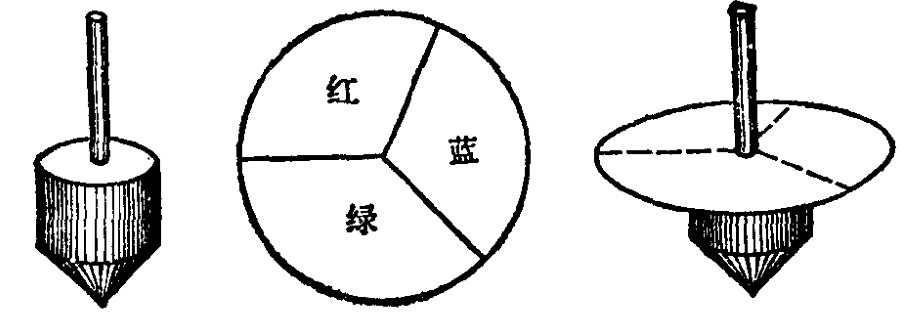
\includegraphics[width=0.6\textwidth]{../pic/czwl2-ch1-35}
    \caption{}\label{fig:1-35}
\end{figure}

如果改变三色板上三种颜色的深浅程度,当陀螺很快旋转的时候,看到三色板又是另一种颜色。
这样,调配红、绿、蓝三种颜色的深浅,我们便可以得到不同的颜色。


